\chapter{Potential Map}
\label{ch:pot_map}

With an average geometry in-hand, the potential map for the water molecules rotating about the high-symmetry point can be investigated, which is the primary focus of this chapter. To begin, a broad sweep is conducted to confirm energy convergence, verify that the antiferroelectric coupling is energetically favorable, and to determine a smaller range for a fine sweep that captures all of the interesting features. 

With an acceptable smaller range for the fine sweep identified, a fine sweep is carried out with antiferroelectric coupling both within the beryl framework and in vacuum. Furthermore, a fine sweep potential map is measured in vacuum with the beryl-based water molecule geometry as found in the previous chapter. 

In the final subsection, the differences in the fine sweep potential map are analyzed to determine (a) if the \textit{interesting} features of the potential maps are products of interaction in the water-beryl or water-water subsystems and (b) what the contribution is of the water-beryl subsystem interactions to the total potential map.

    \section{Motivation for Investigation}
    
    \begin{figure}
        \centering
        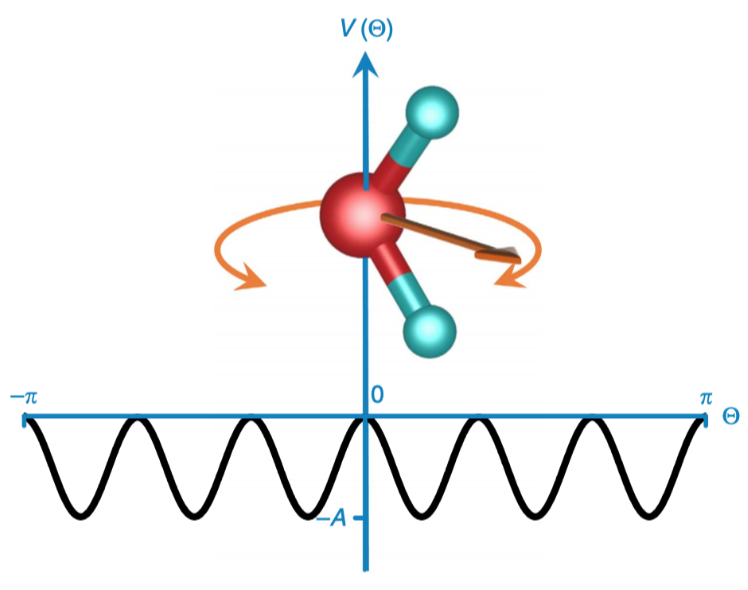
\includegraphics[width=0.7\linewidth]{Figures/System/pmap_misha.png}
        \caption{Assumed six-fold sinusoidal potential map. [\textbf{vibrational paper}]}
        \label{fig:pmap_misha}
    \end{figure}
    
    Before beginning, however, it is important to highlight exactly why the seemingly contrived high-symmetry potential map is worth investigating.
    
    First and foremost, there is discrepancy in the literature about what the potential map looks like. Some groups have assumed a six-fold sinusoidal potential map (Fig. \ref{fig:pmap_misha}) [\textbf{vibrational paper}]. No distinction is made as to which rotation configuration the minima correspond. Another group has utilized a less-strict assumption \textemdash namely, a six-fold degenerate harmonic expansion (Fig. \ref{fig:pmap_other}). While here the minima are assigned to aligned nearest-neighbors, the potential in between minima is assumed to be constant. 
    
    Both assumed potential maps have been used in the analysis of data from optical experiments. If a more accurate potential map can be used, the results from said analyses should improve.

    \begin{figure}
        \centering
        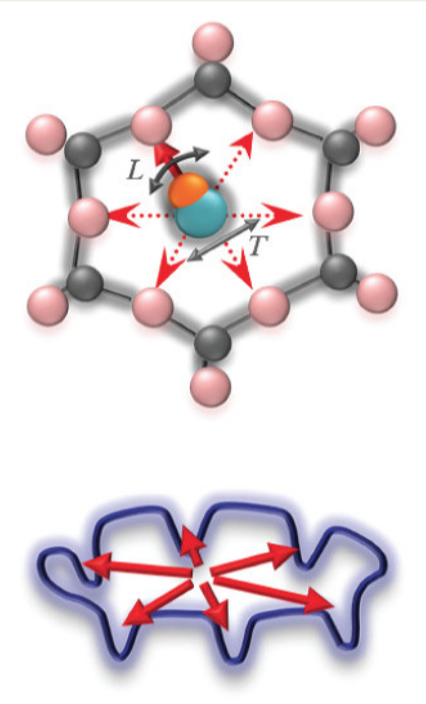
\includegraphics[width=0.5\linewidth]{Figures/System/pmap_other.png}
        \caption{(Top) Top-down view of water molecule in nanocage with transverse and librational modes identified. (Bottom) Assumed potential map using six-fold degenerate harmonic expansions. [\textbf{other_pmap_papers}]}
        \label{fig:pamp_other}
    \end{figure}
    
    Furthermore, the potential map, specifically the \textit{groundstate} potential map, provides a nice point-of-comparison for any future coarse-grained force fields and would allow for easy parameter tuning.

    \section{Broad Sweep}
    Like one would do when surveying a new region, a broad sweep is first carried out to set bearings, test a assumptions, and begin to understand how both fill and rotation of the water molecules affects the energetics of the system. 
        \subsection{Energy Convergence Test}
        \label{sec:en_conv_test}
        \paragraph{Procedure} As was done with the structural optimization, the convergence of the relevant parameter--here, potential energy--is first tested. In previous works, energy barriers for the water molecule librations are reported to be fraction of meV \cite{vibr_states}. To recall, an energy difference tolerance of $10^{-4}$ eV for the structural optimization. Again, for reasons of computational cost, using this tolerance is ideal, but it is on the order of the features intended to be measured. Therefore, the potential map under this energy difference tolerance is compared to that obtained under a tolerance of $10^{-6}$ eV. 
        
        For the larger tolerance, the configuration for fill 1010 is used. The two extra-framework water molecules are coupled ferroelectrically---meaning the relative angle between molecules vanishes at all times---and starting from the standard position, are rotated through $\pi$ radians in steps of $\Delta \theta = \pi/150$. The resulting potential map is then inspected (see Fig. \ref{fig:pmap_convergence}) to determine a slightly smaller rotation range for the smaller tolerance that still maps the features of interest, since the computation time for said smaller tolerance is significantly longer. Using this smaller range of $\pi/3$ radians with the same $\Delta \theta$, the ferroelectrically coupled water molecules are again rotated, and the potential map is measured.
        
        The comparison of these maps is carried out via the ratio of the energies for each angle $\theta \in \{0,\pi/3\}$. Again, assuming that the results are not significantly difference, the ratio should approach unity for each rotated configuration.
        
        \paragraph{Calculation Details} For each rotated configuration, the standard self-consistent calculator is used, with the only difference being the energy difference tolerance EDIFF as out discussed above.
        
        \paragraph{Results and Analysis}
        
        \begin{figure}
            \centering
            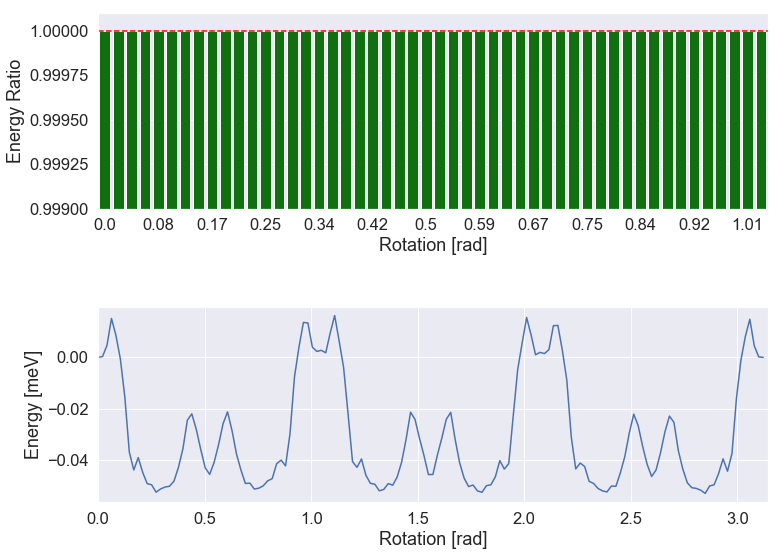
\includegraphics[width=0.8\linewidth]{Figures/System/pmap_convergence.png}
            \caption{The results for the energy convergence test. (Top) The ratio of the energies calculated under both energy difference tolerance for each rotated configuration. The dashed, red line indicated unity. (Bottom) The broad sweep potential map under energy difference tolerance $10^{-4}$ eV. See text for analysis. }
            \label{fig:pmap_convergence}
        \end{figure}
        
        The results for the energy convergence test are shown in Fig. \ref{fig:pmap_convergence}. As evident from the top subfigure therein, no appreciable accuracy in the potential energy calculation is gained from the smaller energy difference tolerance. For each angle of rotation, the ratio is exactly unity, at least within the resolution of the graph. The larger tolerance is therefore deemed acceptably converged for purposes of calculating potential maps.
        
        The bottom subfigure in Fig. \ref{fig:pmap_convergence} shows the broad sweep potential map. Immediately, some relevant features are identifiable. Specifically, there are two sets of 6-fold degenerate local minima. The first of these two local minima appear at $\theta = n\pi/3$ for $n\in \left[0,5\right] \cap \mathbb{Z}$. These angles correspond to positions where the water molecule dipole moment is coincident with the dipole moment of a nearest neighbor water molecule. (See Fig. \ref{fig:supercell} for visual aid.) Offset from these minima by $\Delta \theta = \pi/6$ radians are the second set of local minima, which correspond to dipole coincidence amongst next-nearest neighbors. 
        
        Additionally, there exists a 12-fold degenerate global minimum in-between the two above described local minima and other shoulder features within the potential map. These will be examined in further detail under the fine sweep, along with an attempt to determine the originating interactions for said features.
        
        \begin{figure}
            \centering
            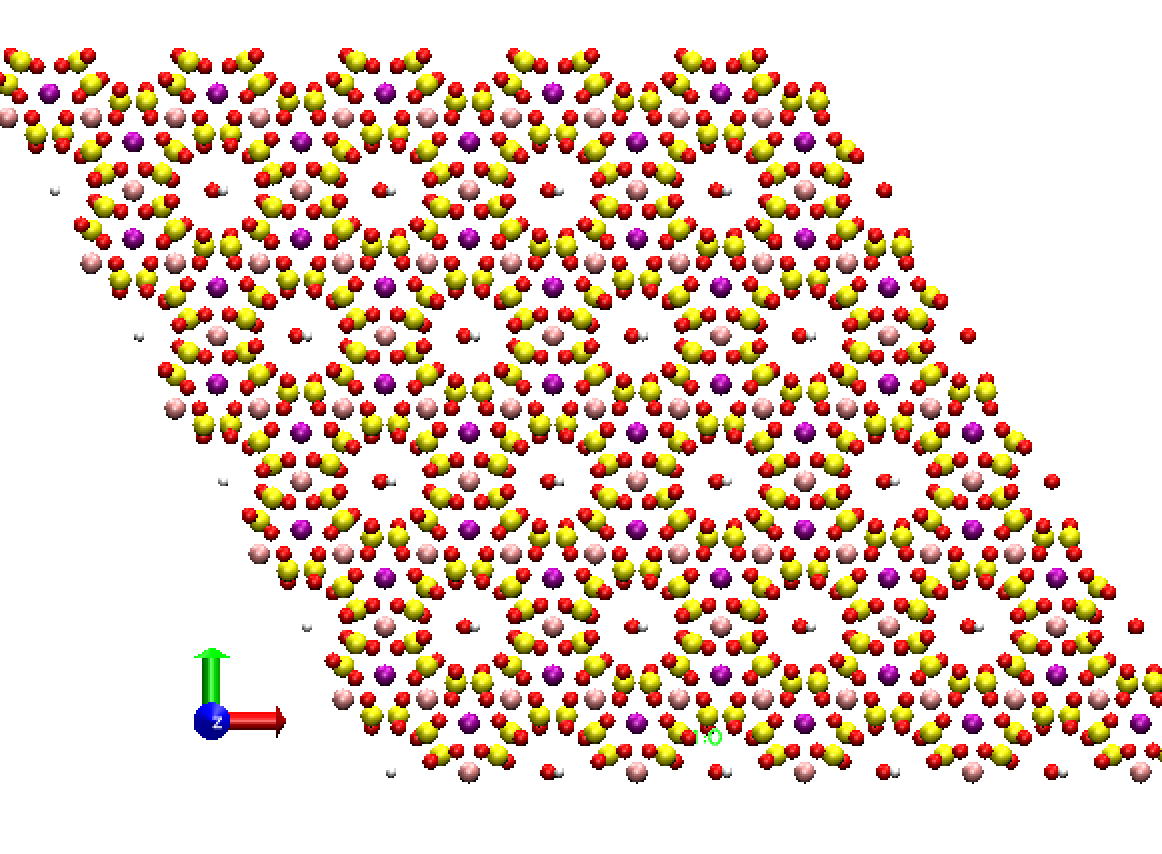
\includegraphics[width=0.8\linewidth]{Figures/System/supercell.png}
            \caption{Large supercell of ferroelectrically coupled fill 1010 system.}
            \label{fig:supercell}
        \end{figure}
        
        \paragraph{Conclusions} The above results are consistent with existing studies that utilized the potential map in some fashion \cite{vibr_states} [\textbf{CITE OTHER PMAP ARTICLE}] in the sense that there does exist a 6-fold degenerate local minimum that corresponds to symmetric rotation configuration about the high-symmetry point. However, thus far an ambiguity has been raised, because it is not clear \textit{which} of the two 6-fold degenerate minima the previous works are referring. Once a fine sweep is conducted, energy barriers can be measured, and hopefully this ambiguity can be lifted.
        
        For the remainder of the broad sweep investigation and in the interest of speeding up data set collection times, a smaller rotation of $\pi/3$ radians is deemed appropriate to capture the three minima and other relevant features. 
        
        \subsection{Relative Angle Test}
        \label{sec:rel_ang_Test}
        
        \paragraph{Background Information }Moving forward, choices need to be made to limit the portion of the parameter space that is sampled due to resource limitations. Since the ultimate goal is to develop a parameterized force field that can capture the groundstate interactions of the extra-framework water molecules, limiting the calculated potential maps to those that correspond to the most energetically favored state is one such choice. If the contributions from the framework crystal are truly of the static variety, then thinking of the water-water subsystem as two identical, interacting classical dipoles in vacuum is a useful heuristic. If said dipoles are interacting in the same fashion as the two water molecules in the crystal, the only relevant degree of freedom is rotation about the c-axis, and the interaction is described by
        
        \begin{equation}
        \label{eq:dip_interaction}
            V(\theta) = k\frac{p^2\cos \theta}{r_0^3},
        \end{equation}
        
        \noindent for some constant of proportionality $k$, dipole moment $p$, separation distance $r_0$, and relative angle $\theta$. Equation \ref{eq:dip_interaction} is minimized when $\theta = \pi$, or when the two dipoles are antiferroelectrically coupled. 
        
        \paragraph{Procedure} Sticking with the fill 1010 configuration, potential maps through rotation angle $\pi/3$ radians with $\Delta \theta = \pi/90$ are calculated where the relative angle between the water molecules $\alpha$ is varied. The relative angles investigated are $0 \le \alpha \le \pi$ in increments of $\Delta \alpha = \pi/6$.
        
        \paragraph{Calculation Details} As before, the standard self-consistent calculator is used for each configuration listed above.
        
        \paragraph{Results and Analysis}
        
        The results of the relative angle test are given in Fig. \ref{fig:pmap_rel_angle}. Immediately, it's clear that the potential maps are qualitatively equivalent not only to each other, but also to the results of the convergence test (Fig. \ref{fig:pmap_convergence}). Specifically, the degeneracy previously identified are present for each relative angle configuration. 
        
        \begin{figure}
            \centering
            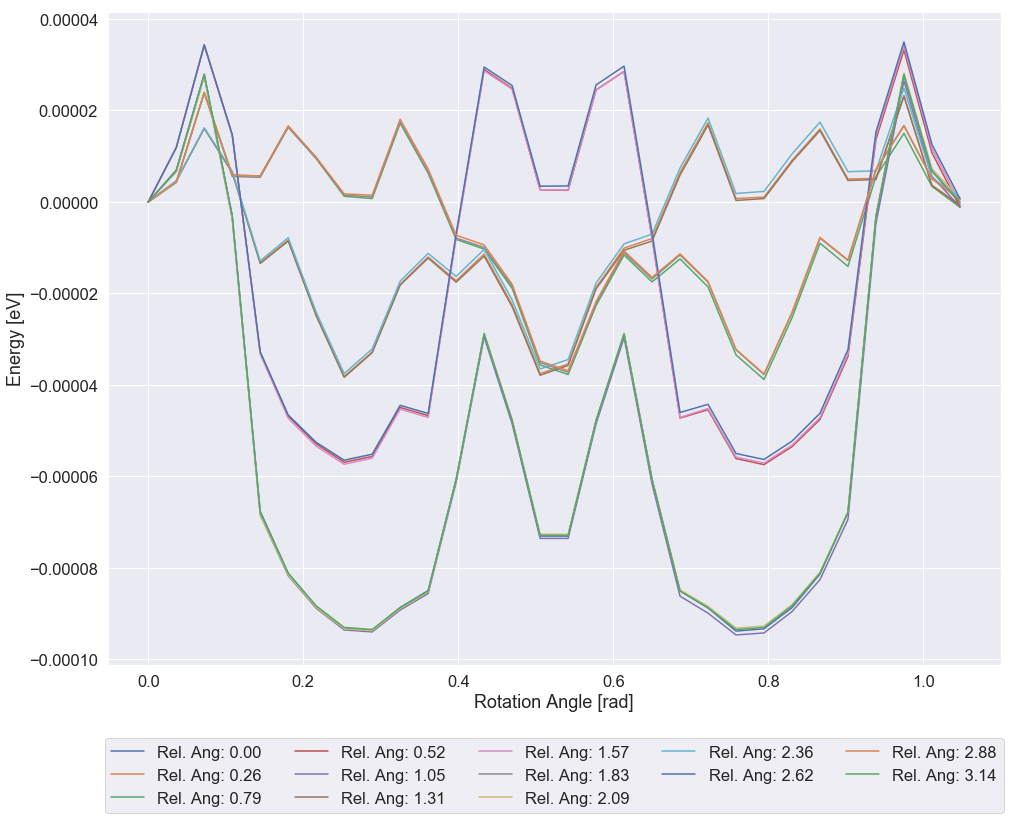
\includegraphics[width=0.9\linewidth]{Figures/System/pmap_rel_angle.png}
            \caption{The potential maps for various relative angle between water dipoles $\alpha$. See text for analysis.}
            \label{fig:pmap_rel_angle}
        \end{figure}
        
        Turning now to the differences between the relative angle potential maps, it is clear from inspection that the antiferroelectrically coupled configuration is the most energetically favorable. Furthermore, the potential map appears to experience a non-linear, negative shift as relative angle increases. There also appear to be differences in the \textit{topology} of the potential maps. 
        
        A more quantitative analysis of the changes described above entails comparing the results to (\ref{eq:dip_interaction}) by answering the question, how does the potential map behave as molecule A is held fixed while molecule C rotates? To answer this question, vertical line cuts of Fig. \ref{fig:pmap_rel_angle} are made using the following procedure for each rotation angle $\theta_i$. The energy difference between $E(\theta_i,\alpha_j)$ for relative angle $\alpha_j$ and $E(\theta_i,0)$ is determined for each $\theta_i$ and $\alpha_j$. Then, the average is taken over all $\theta_i$, resulting in an average description of the energy as a function of relative dipole angle $\alpha$ that should be approximated by (\ref{eq:dip_interaction}). The results are shown in Fig. \ref{fig:relative_angle_fit}. Here, the function is fit by hand to 
        
        \begin{equation}
            E(\alpha) = A \sin(\omega \alpha),
        \end{equation}
        
        \noindet with amplitude $A = -0.88$ meV and frequency $\omega = \pi/6$. The function was fit by hand due to the difficulties of fitting a sinusoidal function only one-half wavelength's worth of data. Even with such a rudimentary fit protocol, though, it is clear that the data agrees reasonable well with (\ref{eq:dip_interaction}), with deviations (specifically below 1.0 radians) being attributed to dipole-framework and higher order dipole-dipole interactions that are not captures by the heuristic assumption. The need for error bars---representing the standard error of the mean---further suggests that the dipole-framework and higher order dipole-dipole interactions influence the potential map topology. Put differently, the distinguishable features of the potential map should vary with relative angle.
        
        \begin{figure}
            \centering
            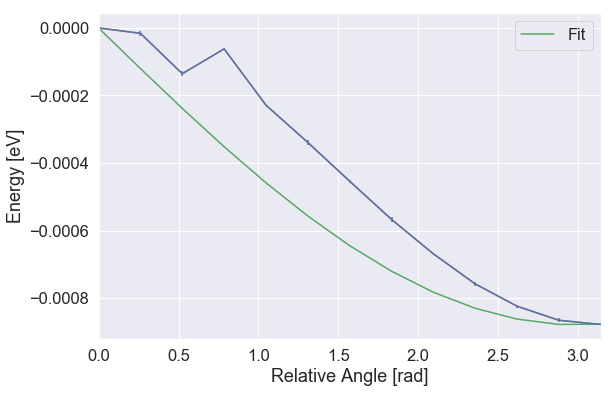
\includegraphics[width=0.9\linewidth]{Figures/System/relative_angle_fit.png}
            \caption{The average energy as a function of relative angle $\alpha$ is compared to a sine function. See text for details.}
            \label{fig:relative_angle_fit}
        \end{figure}
        
        This variation is captured when each potential map in Fig. \ref{fig:pmap_rel_angle} is zeroed relative to the energy in the initial configuration, as shown in Fig. \ref{fig:zeroed_relative_angle_pmap}. In general, the two 6-fold degeneracies and one 12-fold degeneracy are visible for each relative angle, but the energetic of these features varies with relative angle. 
        
        \begin{figure}
            \centering
            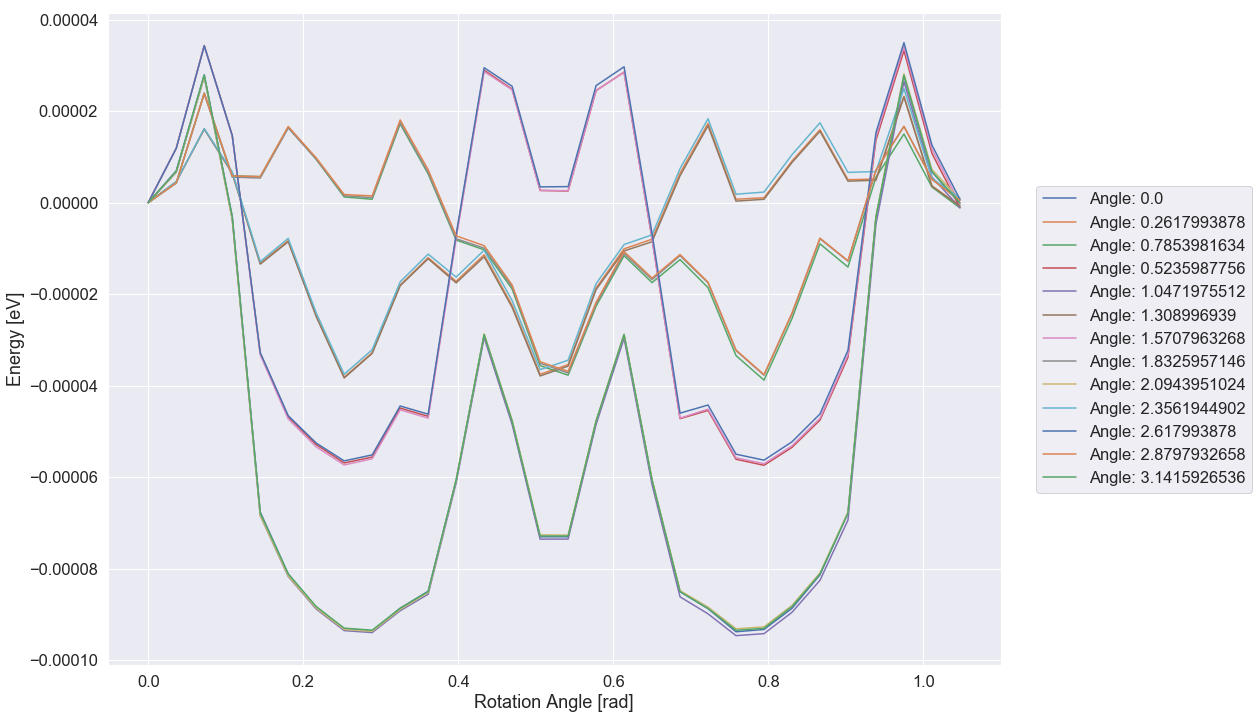
\includegraphics[width=0.9\linewidth]{Figures/System/pmap_zeroed_relative_angle.png}
            \caption{Relative angle potential maps zeroed relative to the energy of the initial configuration.}
            \label{fig:zeroed_relative_angle_pmap}
        \end{figure}
        
        \paragraph{Conclusions} Finally, the antiferroelectrically coupled configuration, as predicted by the heuristic assumption, is in fact the most energetically favorable and allows for a reduction in parameter space. Using this reduced parameter space, the effect that additional water molecules have on the potential map can be investigated by determining the antiferroelectrically coupled map for each fill configuration.
        
        \subsection{Map vs. Fill}
        \label{sec:map_v_fill}
        
        \paragraph{Procedure} Similar to the relative angle test procedure, potential maps are calculated for each fill using antiferroelectrically coupled water molecules. The molecules are rotated through $pi/3$ radians with $\Delta \theta = pi/90$. To make a meaningful comparison between fills, each potential map is zereoed to the energy of the initial configuration.
        
        \paragraph{Calculation Details} The standard self-consistent calculated is used.
        
        \paragraph{Results and Analysis}
        
        \begin{figure}
            \centering
            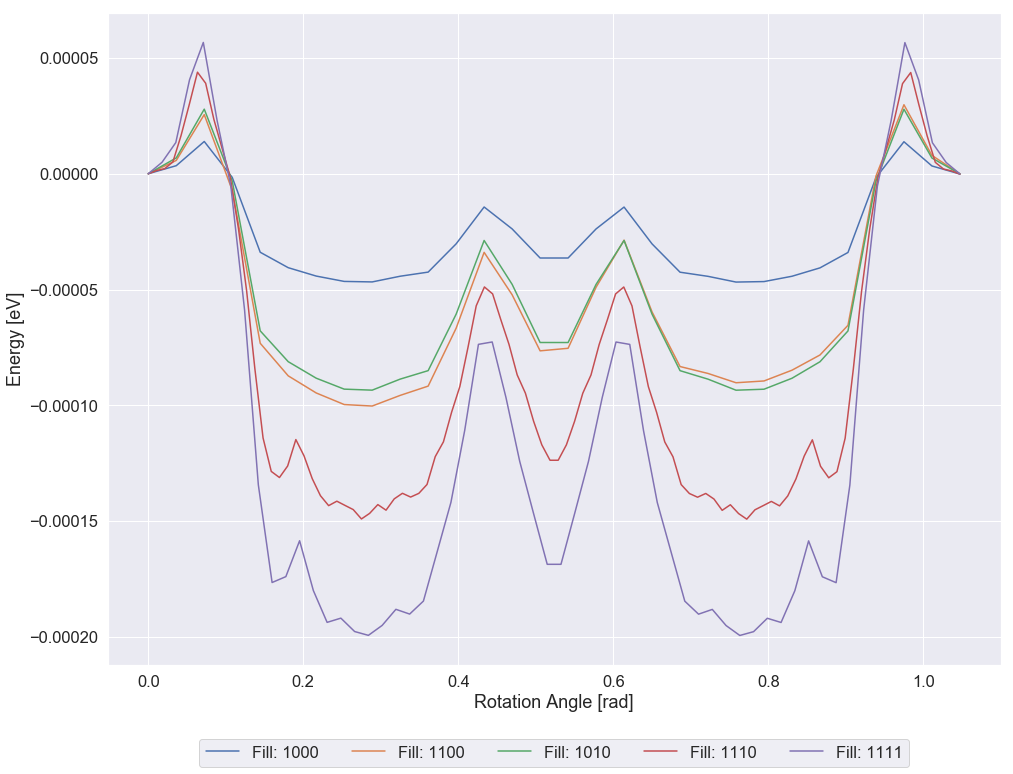
\includegraphics[width=0.9\linewidth]{Figures/System/pmap_af_broad.png}
            \caption{The antiferroelectrically coupled potential maps as a function of fill.}
            \label{fig:pmap_af_broad}
        \end{figure}
        
        Figure \ref{fig:pmap_af_broad} shows the potential maps as a function of fill. The interesting features, namely the already-described degeneracies, are evident in each fill (although some of the smaller shoulders are not visible within the resolution of the graph). As more water molecules are added, the potential wells deepen. Also, by comparing the local minima to the crystal symmetry, the minima correspond to instances when the water molecules are colinear with nearest- or next-nearest-neighbor water molecules. It is unclear at this point, however, if the features should be attributed to dipole-dipole interaction or dipole-framework interactions. The next section will attempt to probe this ambiguity by performing a fine sweep over $0\le \theta \le 0.6$ radians, which will capture all relevant features shown in Fig. \ref{fig:pmap_af_broad}. To try to disentangle the dipole-framework and dipole-dipole interactions, potential maps will also be calculated for arrays of water molecules in vacuum with the same spacing as if the crystal were present.
        
        Before moving on, however, it is also useful to look at how the average energy of the system changes as a function of fill. By averaging the total energies over configurations for each fill, the effect that adding water molecules to the crystal can be ascertained. These results are depicted in Fig. \ref{fig:pmap_avg_energy}. Here, the results for the degenerate $\phi = 0.5$ case are combined.
        
        It is clear that there is a well-defined inverse, linear relationship between the number of water molecules and the total energy of the system. It is worth remembering at this point, though, that the geometry of the crystal framework was held constant for all calculations, so the true relationship might deviated slightly from near-perfect linearity. 
        
        From fitting the data to 
        
        \begin{equation}
            y = -57.28x+14.32 \text{ with } x = \frac{n_\text{w}}{4},
        \end{equation}
        
        \noindent with number of water molecules $n_\text{w}$, the addition of each water molecule decreases the total energy by 14.3125 eV. Thus, it is energetically favorable for a beryl crystal to have every cage filled with a water molecule.
        
        It would be interesting to see how Fig. \ref{fig:pmap_avg_energy} would look using a larger unit cell with greater fill degeneracies, since such a curve would more accurately describe nature. Such large unit cells would be extremely expensive to calculate and would require greater computational resources than were available at time of research.
        
        \begin{figure}
            \centering
            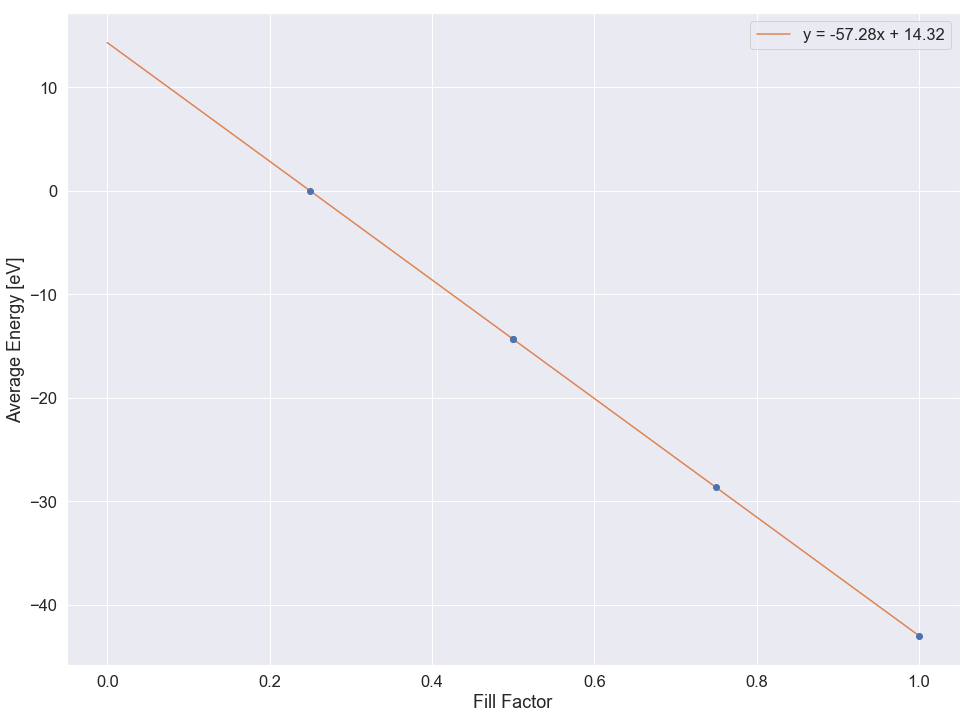
\includegraphics[width=0.9\linewidth]{Figures/System/pmap_broad_avg_energy.png}
            \caption{The average energy as determined by the self-consistent calculation for each fill. The error bars, which are not visible within the resolution of the graph, represent the standard-error of the mean.}
            \label{fig:pmap_avg_energy}
        \end{figure}
        
        
        
    \section{Fine Sweep}
    \label{sec:fine_sweep}
    
    The broad-sweep potential maps offer enlightening insights into the energetics of the beryl-water system but much of the results are qualitative in nature. For instance, how does the energy difference between the local minima change \textit{quantitatively} as a function of fill? Furthermore, are the distinguishable features of the potential map due to dipole-dipole or dipole-framework interactions? 
    
    \paragraph{Procedure} To answer these questions, potential maps will be calculated over a smaller range with greater resolution for two cases: (a) the water molecule arrays are within the beryl crystal and (b) the water molecule arrays are in vacuum but with the same spacing as in case (a). For case (b), potential maps will be calculated with two different water molecule geometries: (1) the vacuum geometry and (2) the beryl geometries as described in Section \ref{sec:geom_opt}. For each case, the water molecules will be antiferroelectrically coupled and rotated through $0\le \theta \le 0.6$ with $\Delta \theta = 0.01$. 
    
    Finally, by taking the difference between pairs of these three potential maps, an attempt is made to disentangle the dipole-dipole and dipole-framework interactions.
    
    \paragraph{Calculation Details} The self-consistent calculator is used for all calculations.
    
        \subsection{In Beryl}
        \label{sec:fine_sweep_beryl}
        
        Figure \ref{fig:pmap_fine_sweep} shows the fine-sweep potential maps as well as five critical points A-E as indicated by vertical lines. Points A, C, E are local minima while points B, D are local maxima. The critical points were determined by finding the local minimum/maximum amongst the sampled points in the neighborhood of the visually identifiable critical points. Thus, these points are approximations of the true critical points, with the accuracy improving with smaller sample frequencies. 
        
        
         \begin{figure}
             \centering
             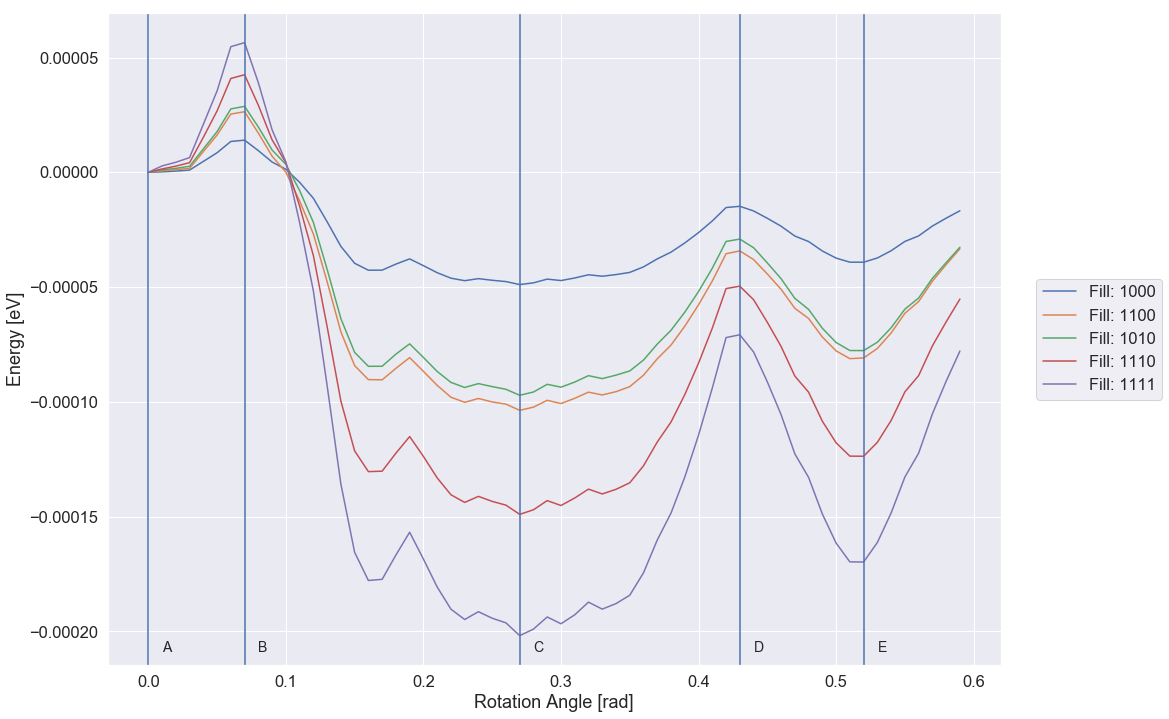
\includegraphics[width=0.9\linewidth]{Figures/System/pmap_fine_sweep.png}
             \caption{Fine-sweep potential maps for each fill with five critical points A-E identified by vertical lines.}
             \label{fig:pmap_fine_sweep}
         \end{figure}
         
         Nevertheless, quantitative information can be obtained about the effect of adding additional water molecules by comparing the energy differences between critical points, as shown in Fig. \ref{fig:pmap_cp_diff}. Here, the relative differences amongst the local minima A, C, E (respectively at points A, C, E) are compared as a function of fill, and the dilating effect of adding additional water molecules is clearly visible by the greater absolute difference in energy between all minima. 
         
         Figure \ref{fig:pmap_cp_diff} also identifies a source of systematic error in that the intercepts do not all vanish. This is possibly due to calculation-approximation systematic errors---such as tolerances, basis sets, functionals, etc.---or more likely due to the finite,small unit cell. Looking at the only degenerate case $\phi=50$, there is slight difference in the results due to the different configurations, and thus an aggregate value must be used. In the limits of an infinite unit cell and of sampling all degenerate configurations, this error would likely be eliminated. There is the possibility that the intercept may not truly vanish, though, which would indicate that some contribution from the dipole-framework exists as well.
         
         \begin{figure}
             \centering
             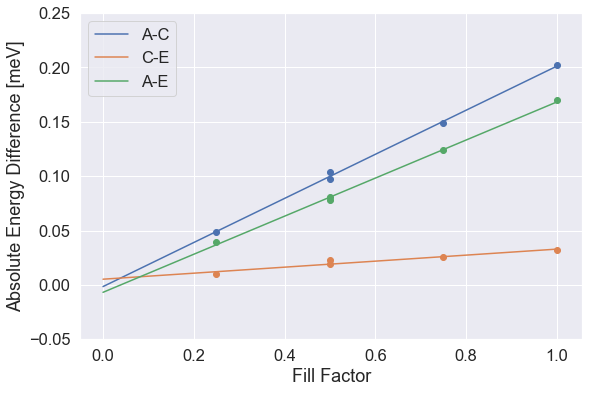
\includegraphics[width=0.9\linewidth]{Figures/System/pmap_cp_diff.png}
             \caption{The difference in energy between the local minima as a function of fill.}
             \label{fig:pmap_cp_diff}
         \end{figure}
         
         The critical point analysis may also hint at a way to dramatically improve experimental investigations of these systems. As it stands, if one wanted to conduct fill-based analysis on an observable, say dielectric response, they must first perform all necessary spectroscopic experiments before determining the fill via mass spectrometer. All the while hoping that the sample they are working with has the fill that they want. On the other hand, if some type of scattering experiment were able to resolve any of the energy differences between local minima, future researchers would be able to approximate their system's fill by performing such a scattering experiment, virtually eliminating the aforementioned experimental bottleneck.
         
         Finally, the fact that the absolute energy differences nearly all vanish suggests that the potential map features are primarily due to interactions within the dipole-dipole system. To elucidate this observation, similar analysis is performed on the vacuum potential maps.

        \subsection{In Vacuum}
        \label{sec:fine_sweep_Vacuum}
        
        Using the vacuum potential maps in Fig. \ref{fig:pmap_vacuum_comparison}, the dipole-dipole and dipole-framework interactions can begin to be disentangled. In said figure, the solid, colored line represent the potential map of an array of water molecules with spacing as if they were within the framework crystal but with the vacuum internal geometry. Because it was shown that the crystal has an effect on the geometry of the water molecule, vacuum potential maps where also calculated using the beryl internal geometry. These latter results are represented by the dotted, black lines. From inspection, it is clear that the beryl geometry slightly raises the energy systematically. but the distinguishable features remain qualitatively unchanged.
        
        \begin{figure}
            \centering
            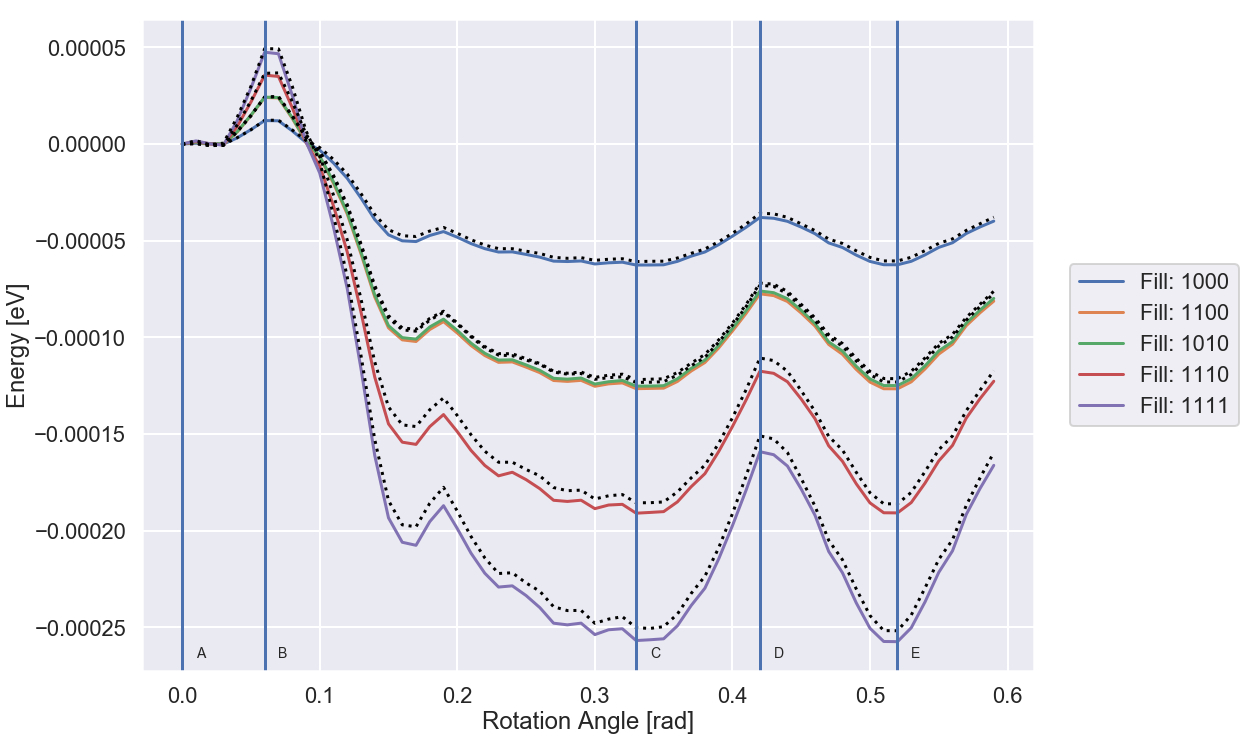
\includegraphics[width=0.9\linewidth]{Figures/System/pmap_vacuum_comparison.png}
            \caption{Potential map by fill for arrays of water molecules in vacuum. The solid, colored lines represent results for water molecules with vacuum geometry, while the black, dotted lines represent results for water molecules with beryl geometry. Critical points are identified as before.}
            \label{fig:pmap_vacuum_comparison}
        \end{figure}
        
        The critical points are determined using the same protocol as in the beryl case. It is worth noting that the angle at which these critical points occur differs from that of the beryl case. For instance, in the absence of the beryl crystal, critical point B is shifted to the left, while critical point C is shifted to the right. Since these represent a local maximum and a local minimum respectively, this suggests that the dipole-framework interactions yield a slight increase in energy. This observation will be discussed in more depth in the Difference Analysis section.
        
        \begin{figure}
            \centering
            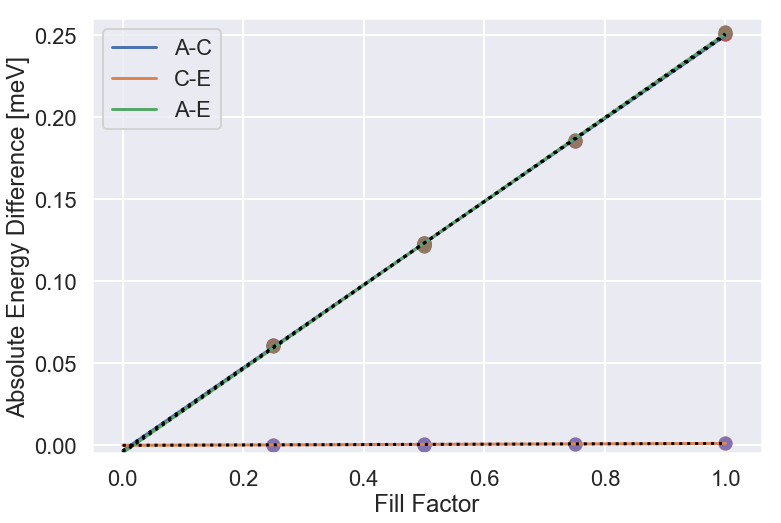
\includegraphics[width=0.9\linewidth]{Figures/System/pmap_vacuum_cps.png}
            \caption{The absolute energy differences are various critical points for the vacuum potential maps. Again, the solid, color lines represent results for vacuum-geometry water molecules, while the dotted, black lines represent the results for beryl-geometry water molecules.}
            \label{fig:pmap_vaccum_cps}
        \end{figure}
        
        Before moving on to the difference analysis, the difference in absolute energy between critical points A, C, and E is examined as in the beryl case (Fig. \ref{fig:pmap_vaccum_cps}. As mentioned in the caption, the same line-style convention is used as in Fig. \ref{fig:pmap_vacuum_comparison}. There exists no distinguishable difference between the vacuum-geometry and beryl-geometry water molecules. There is, however, a striking difference between these results and those shown in Fig. \ref{fig:pmap_cp_diff}. Namely, there is a degeneracy in the vacuum case that appears to be lifted within the present of the crystal framework. In Fig. \ref{fig:pmap_vaccum_cps}, The difference in energy between point A and points C, E are the same, while the difference between points C, E appears to vanish. This suggests that a degeneracy exists for the global minimum at points C and E. The lifting of this degeneracy supports the previous finding that the crystal acts as a non-interacting, background potential.
        
        One further point on the degeneracy here: It is known that in the case of a one-dimensional chain of spins in vacuum no phase transition occurs with respect to their alignment \textbf{[citation needed?]}. It may be this degenerate groundstate that plays a role in suppressing such a phase transition, at least in the case of water molecules with the current spacing. Since this degeneracy is lifted in the crystal framework, perhaps a one-dimension chain could exhibit a phase transition. At the very least, it warrants greater investigation.
        
        \subsection{Difference Analysis}
        \label{sec:diff_anal}
        
        There are two ways that information about that the dipole-framework interactions can be disentangled using the potential map data. The first to look at how the critical points shift in the potential map when going from the vacuum case to the beryl case, as shown in Fig. \ref{fig:cp_diff}. Both local minima A and E---corresponding to dipoles being co-linear with the nearest- and next-nearest neighbors, respectively---appear to be unchanged by the addition of the crystal framework. However, the local minimum C experiencing a significant shift to the left when the framework is included. Similarly, the local maxima B and D are both shifted to the right. Both of these shifts are consistent with a static background potential that is directly proportional to the rotation angle over the range calculated. Considering the six-fold symmetry of the system, this background potential likely also exhibits a six-fold potential.
        
        \begin{figure}
            \centering
            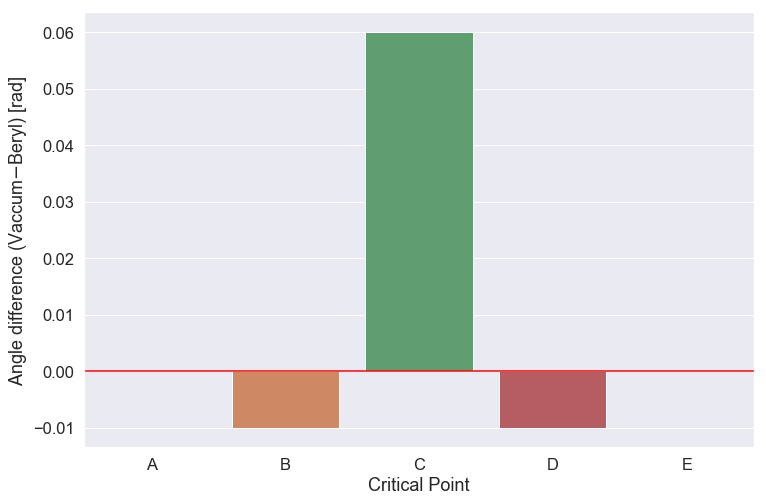
\includegraphics[width=0.9\linewidth]{Figures/System/cp_diff.png}
            \caption{The difference of angles at which the critical points occur. Here, a negative (positive) value indicates that including the framework shifts the critical point to the right (left).}
            \label{fig:cp_diff}
        \end{figure}
        
        The second avenue of investigation provides greater quantitative insight into this static, background potential. By taking the difference in energy between the beryl potential map and the vacuum potential map (with beryl-geometry water molecules), the energy contribution due to the dipole-framework interactions can be determined---this is shown in Fig. \ref{fig:framework_contrubtion}. The results are consistent with those arrived at by examining the critical point shift. That is, the crystal provides a sinusoidal-like increase in energy as the rotation angle increases. Furthermore, since this map is slightly more than half of a sixth of a full rotation, this potential has a six-fold degeneracy, consistent with the symmetry of the crystal. 
        
        \begin{figure}
            \centering
            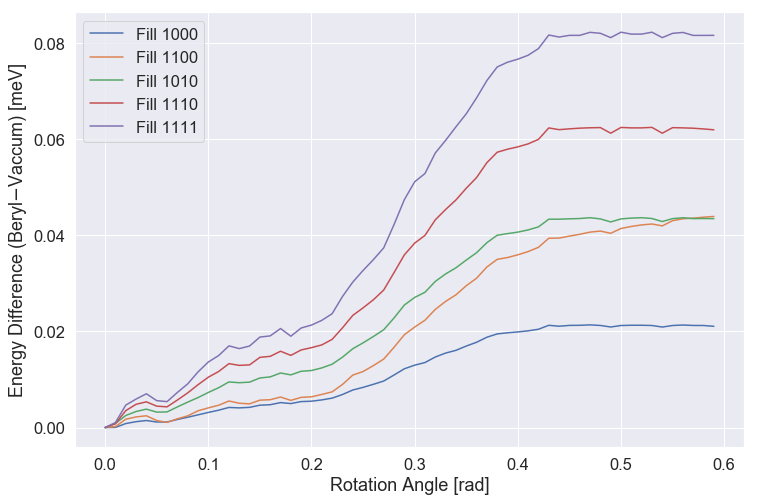
\includegraphics[width=0.9\linewidth]{Figures/System/diff_analysis.png}
            \caption{The difference in potential maps between the beryl and vacuum cases. For consistency, the beryl-geometry water molcules are used for the vacuum case..}
            \label{fig:framework_contrubtion}
        \end{figure}
        
        Also apparent from Fig. \ref{fig:framework_contrubtion} is the fact that fill is not the only relevant parameter for determining the dipole-framework interaction. As evident by the difference in the degenerate $\phi = 0.5$ cases, the specific placement of water molecules is also important. With hopes of trying to find a general relationship, say energy contribution per water molecule, the dipole-framework maps are scaled by the total number of water molecules.
        
        \begin{figure}
            \centering
            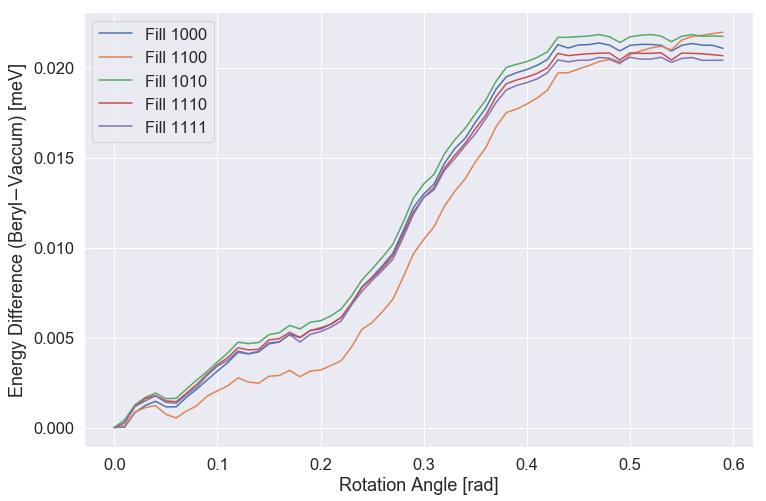
\includegraphics[width=0.9\linewidth]{Figures/System/framework_contribution_scaled.png}
            \caption{The dipole-framework potential maps from Fig. \ref{fig:framework_contrubtion} with the energy scaled by the total number of water molecules.}
            \label{fig:framework_contribution_scaled}
        \end{figure}
        
        Figure \ref{fig:framework_contribution_scaled} shows that the scaled dipole-framework potential maps are beginning to resemble some type of general principle. There is still, however, discrepancies between the individual potential maps, not only between fill types but also degenerate fills as well. This suggests that higher-order dipole-dipole (or even dipole-framework) interactions are relevant. 
        
        Nevertheless, an approximate, general relation can be found by taking the average energy at each rotation angle, as shown in Fig. \ref{fig:framework_contribution_fit}. Here, the error bars represent the standard error of the mean, and a well-defined average energy contribution per water molecule is apparent. Such a feature suggests that a parameterized force-field may be possible in which the framework crystal is coarse-grained away in favor of a rotation-based potential. 
        
        \begin{figure}
            \centering
            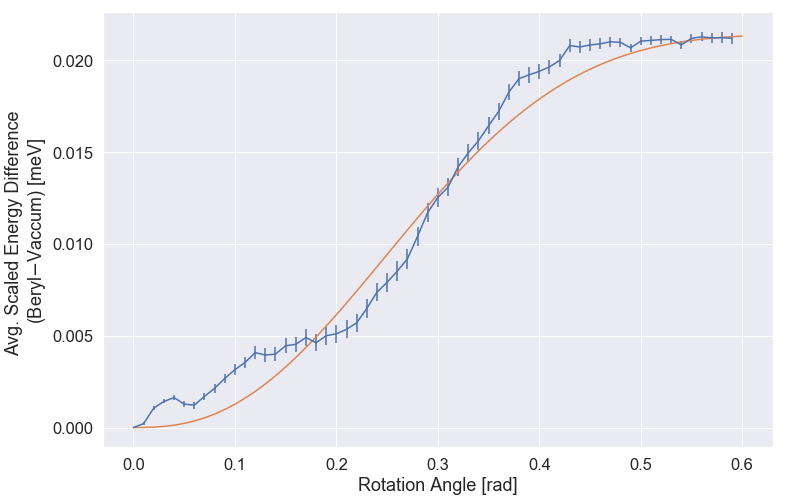
\includegraphics[width=0.9\linewidth]{Figures/System/diff_analysis_fit.png}
            \caption{The average, scaled dipole-framework energy contribution with example of fit. See text for details.}
            \label{fig:framework_contribution_fit}
        \end{figure}
        
        In order for such an approximation to be useful, an analytic function needs to be found, to which the potential map data can be fit. In Fig. \ref{fig:framework_contribution_fit}, a preliminary analytic function is chosen for the fit, specifically
        
        \begin{equation}
        \label{eq:fit}
            E(\theta) = A\sin\left[\frac{\pi}{2} \sin\left( \omega \theta \right)\right]^n,
        \end{equation}

        \noindent for parameters $A,\omega,n$. Equation (\ref{eq:fit}) was chosen after a casual search of sinusoidal functions that exhibit a squished amplitude, but better equations surely exist. Its use here is meant merely to be heuristic in nature. Even still, the fit is decent and hints that this avenue is worth further investigation. 
        
        Besides using an more appropriate analytic function, utilizing a larger unit cell that allows for greater exploration of the fill (and fill-degeneracy) parameter space would yield a more generally appropriate fit. As discussed previously, however, such a large unit cell is cost prohibitive with the resources available for this investigation. Additionally, sampling a full, or at least larger total rotation, within the framework would help in fitting the frequency of analytic function.
        
    \section{Summary and Outlook}
    
    \paragraph{Summary} The Energy Convergence Test (Section \ref{sec:en_conv_test}) provides insights on a few fronts. From a computation standpoint, the larger energy difference tolerance of $10^{-4}$ eV is acceptable for potential map calculations. From a physical standpoint, the calculated potential map tends to agree more with [\textbf{cite pmap2 paper}] in terms of qualitative shape. That is, a six-fold degenerate local minimum occurs when the dipole is co-linear with a nearest-neighbor dipole. In addition, there is a second six-fold degenerate local minimum that corresponds configuration in which the dipole is co-linear with a next-nearest neighbor dipole. In between these two local minima, a 12-fold generate global minimum between the two configurations which does not appear to correspond to any significant case of dipole-dipole alignment.
    
    The Relative Angle Test (Section \ref{sec:rel_ang_Test}) confirms that antiferroelectrically coupled dipole configurations---that is, dipoles with a relative angle difference of $\pi$ radians---are the most energetically favorable. Furthermore, the average energy dependence on the relative angle between dipoles agrees decently with the heuristic
    
    \begin{equation}
    \label{eq:heur}
        E(\alpha) = A \sin(\omega \alpha),
    \end{equation}
    
    \noindent with $A=-0.88$ meV and $\omega = \pi/6$. Deviations from (\ref{eq:heur}) likely represent higher-order dipole-dipole and/or dipole-framework interactions. For the remainder of the investigation, only antiferroelectrically coupled systems are investigated.
    
    In Section \ref{sec:map_v_fill}, the effect that fill has on the potential energy map is investigated. Five fill cases are investigated $\phi \in \{0.25,0.50,0.75,1.00\}$, with a degeneracy in the case of $\phi = 0.50$. As water molecules are added, a dilation effect can be observed in the potential maps. Specifically, the local maxima increase and local minima decrease with each additional water molecule. There is also a noticeable difference between the degenerate $\phi=0.50$ systems, suggesting that relative position of water molecules also plays a role in the energetics, although less significant compared to the effect of fill. In additional the dilation effect, there is a systematic decrease in energy with each water molecule at the rate of $14.3125$ eV/molecule. The fact that the water molecules seem to prefer closer association, at least energetically, is consistent with everyday experiences of water tending to clump together. 
    
    For purposes of disentangling the dipole-dipole interaction from the dipole-framework interactions, a finer range is identified ($0\le\theta\le0.6$) that preserves all distinguishable features and over which a more accurate potential map can be calculated. The results from the Fine Sweep (Section \ref{sec:fine_sweep}) provide the most quantitative insights into the system's energetics. In the beryl case, five critical points A-E are identified that represent the primary local maxima and minima. By looking at the absolute energy difference between said points as a function of fill, a novel method for experimentally determining fill \textit{pre-}experiment is identified, so long as experiment can resolve the energy differences. Examination of the vacuum potential maps pushes this insight further. Again, five critical points are identified that correspond to qualitatively the same maxima and minima. Quantitatively, however, the critical points differ from their beryl-like counterparts in that there is a degeneracy where one did not previously exist. Specifically, points C, E are energetically degenerate. These results suggest that the dipole-framework interaction contributes a static increase in energy. Additionally, there is a difference in the absolute energy of all data points between the vacuum-geometry and beryl-geometry potential maps---the vacuum-geometry is slightly more favorable.
    
    Finally, the differences in these potential maps is analyzed in Section \ref{sec:diff_anal}. First, the angle at which the critical points occur is compared between the vacuum and beryl cases. Both local maxima (B,D) experience a shift towards a higher angle, while the global minimum (C) experiences a shift to a lower angle when the crystal framework is included. This is consistent with the previous assertion about the dipole-framework contribution from the previous section. This contribution is more exactly investigated by taking the difference between the beryl and vacuum cases. As with the previous Map versus Fill test, there is a systematic increase in energy as the fill increases, as well as a lesser dependency on the relative positions of dipoles. When these potential maps are normalized by the total number of water molecules, a more general dipole-framework contribution per water molecule in the average is observed, suggesting that the beryl crystal could be course-grained away assuming a suitable analytic function could be fit to the averaged energy curve. A preliminary function is chosen to demonstrate proof-of-concept
    
    \begin{equation}
    \label{eq:fit}
        E(\theta) = A\sin\left[\frac{\pi}{2} \sin\left( \omega \theta \right)\right]^n,
    \end{equation}
    
    \noindent with $A=0.0214$, $\omega = 2.1772$, and $n=2.5685$$. 
    
    \paragraph{Outlook}
    
    In general, all improvements to the above-described protocols boil down the computational resources. In additional to testing the convergence with respect to energy difference tolerance, testing convergence with respect to cut-off energy, hybrid functionals, etc. would be helpful in bringing the results more inline with nature. Furthermore, a larger unit cell would go a long way in increasing the accuracy of all aggregate results (e.g. being able to sample more fill types and more fill degeneracies). Such a unit cell would also allow for great disentanglement of the energetics, because other relational parameters can be investigated. As it is, though, these would require almost an order of magnitude increase in computational resources.
    
    It would also be interesting to see if a single one-dimensional channel (i.e. only periodic in the $c$-direction) would exhibit a phase transition. If so, it would serve as an example of how a small background perturbation can push a one-dimensional system to a phase transition.